\documentclass[a4paper,12pt]{article}
\addtolength{\oddsidemargin}{-1.cm}
\addtolength{\textwidth}{2cm}
\addtolength{\topmargin}{-2cm}
\addtolength{\textheight}{3.5cm}
\newcommand{\HRule}{\rule{\linewidth}{0.5mm}}
\newcommand\tab[1][1cm]{\hspace*{#1}}
\makeindex
%%%%%%%%%%%%%%%%%%%%%%%%%%%%%%%%%%%%%%%%%%%%%%%%%%%%%%%%%%%%%%%%%%%%
\usepackage{longtable}
\usepackage{graphicx}
\usepackage{makeidx}
\usepackage{hyperref}
\usepackage{verbatim}

\hypersetup{
    colorlinks=true,
    linkcolor=black,
    filecolor=magenta,      
    urlcolor=cyan,
}

\begin{document}


% define the title
\author{Whoosh Division}
\title{OcuViz - EpiUse Labs}
\setlength{\parskip}{6pt}

% generates the title
\begin{titlepage}
\begin{center}
% Upper part of the page       

\includegraphics[scale=1]{../Spec/images/up-logo.jpg}\\[0.4cm]    
\textsc{\LARGE Department of Computer Science}\\[1.5cm]
\textsc{\Large Whoosh Division}\\[0.5cm]
% Title
\HRule \\[0.4cm]
{ \huge \bfseries OcuViz - EpiUse Labs}\\[0.4cm]
\HRule \\[0.4cm]
\begin{minipage}{0.4\textwidth}
\begin{flushleft} \large
Vukile {Langa}
\end{flushleft}
\end{minipage}
\begin{minipage}{0.4\textwidth}
\begin{flushright} \large
\emph{} \\
u14035449 
\end{flushright}
\end{minipage}
\begin{minipage}{0.4\textwidth}
\begin{flushleft} \large
Wynand Hugo Meiring
\end{flushleft}
\end{minipage}
\begin{minipage}{0.4\textwidth}
\begin{flushright} \large
\emph{} \\
u13230795  
\end{flushright}
\end{minipage}
\begin{minipage}{0.4\textwidth}
\begin{flushleft} \large
Nontokozo Hlastwayo
\end{flushleft}
\end{minipage}
\begin{minipage}{0.4\textwidth}
\begin{flushright} \large
\emph{} \\
u14414555
\end{flushright}
\end{minipage}
\begin{minipage}{0.4\textwidth}
\begin{flushleft} \large
Gerome Schutte
\end{flushleft}
\end{minipage}
\begin{minipage}{0.4\textwidth}
\begin{flushright} \large
\emph{} \\
u12031519
\end{flushright}
\end{minipage}
\vfill

{\large \today}
\end{center}
\end{titlepage}
\footnotesize
\normalsize

%
%
%
%
%
%
%	Table of Contents
%

\tableofcontents
\newpage
\setlength{\parindent}{0em}
\section{Introduction}
When presented with fairly large or small numbers we as human beings tend to struggle. One struggles to grasp the sheer magnitude of how much a trillion dollars is for example or the distance light travels in a second.

The aim of OcuViz is to create a platform for the visualization of data in 3D space using virtual reality to provide an immersive and presence depth.

\section{General Information}
\subsection{System Overview}

OcuViz is a platform for the visualisation of data in a virtual 3D space to allow users to conceptualise large numbers more accurately and naturally. Leveraging the power of VR we are able to create awe-inspiring and immersive scenes for users to experience. As well as, allowing users to create their own scenes through either modular CSV files which are interpreted into 3D scenes or a simplified editor without requiring the user having to be a graphics experts.

\subsection{System Configuration}

Minimum hardware requirements to run OcuViz
\begin{itemize}
\item VR Headset:\tab Oculus Rift DK2
\item GPU:\tab[2.1cm] GTX 970 or AMD R9 290
\item CPU:\tab[2.2cm] Intel Core i5-4590
\item RAM:\tab[2.1cm] 8GB
\item USB:\tab[2.3cm] 2 USB 3.0 ports
\item OS:\tab[2.6cm] Windows 7 SP1
\end{itemize}

\newpage

\textbf{Communication diagram} \\
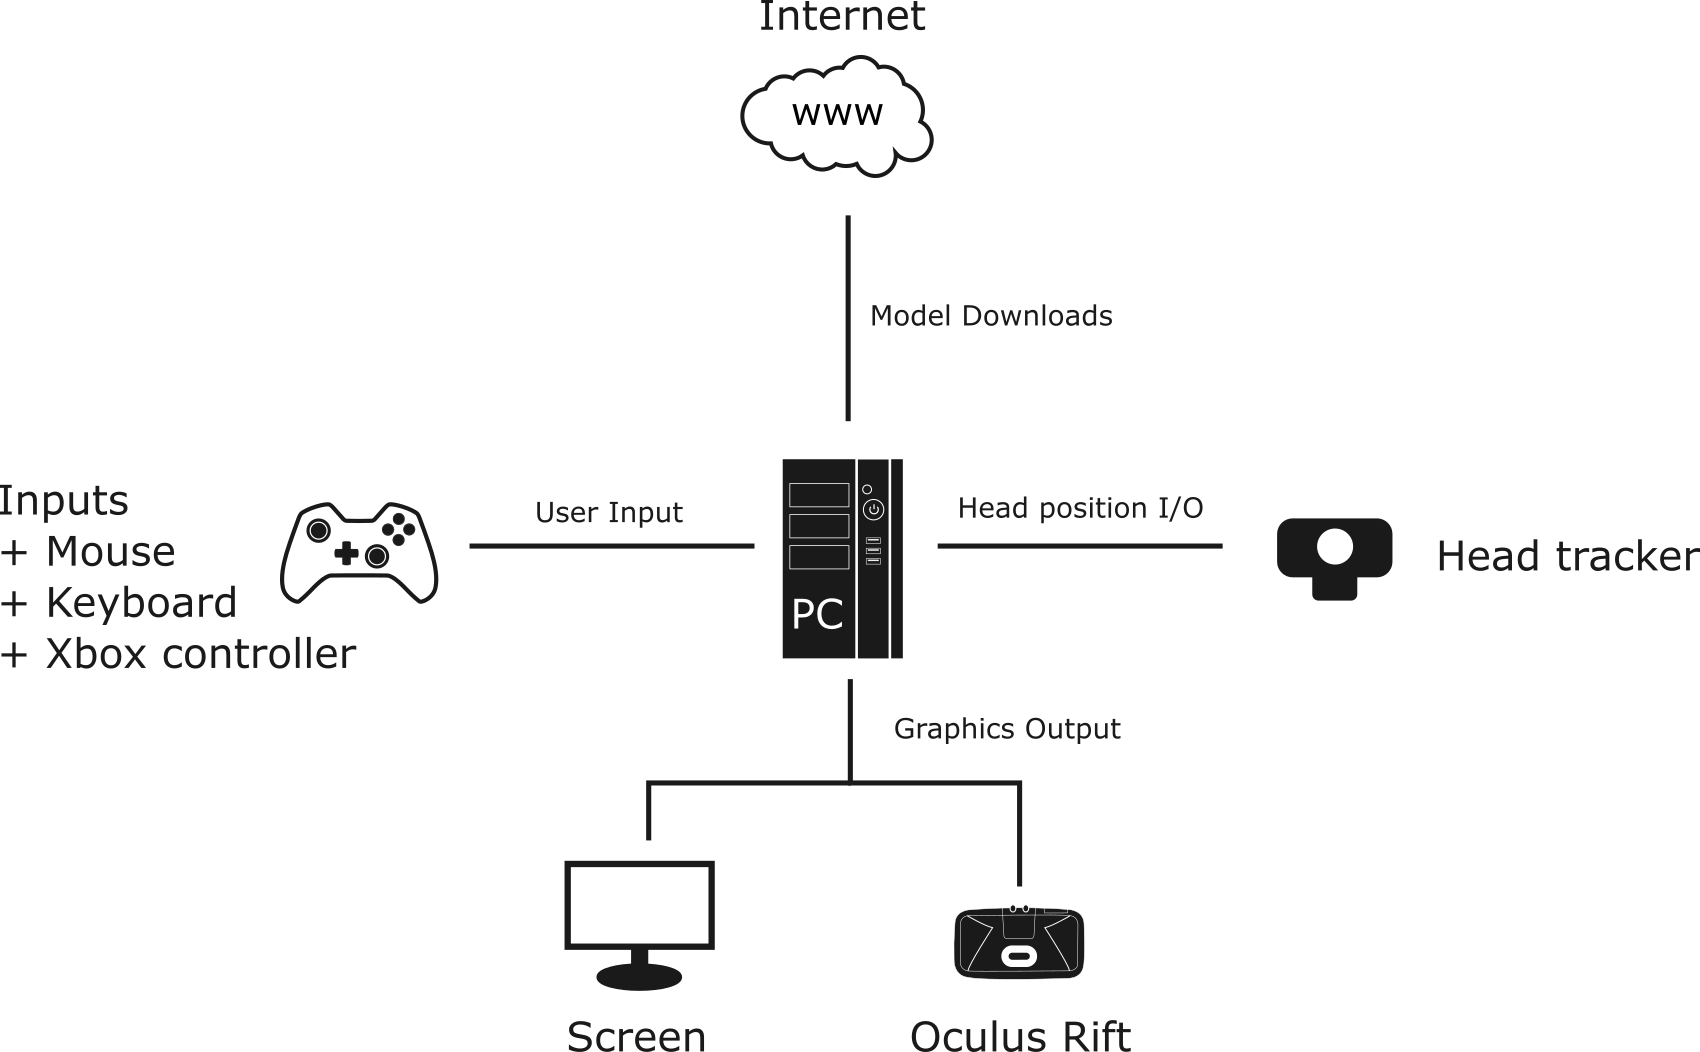
\includegraphics[scale=0.1]{communication.png}

OcuViz receives input from the user through either keyboard, mouse and xbox controller. Or from the head tracker camera which sends location based input to OcuViz with regards to user height, head orientation, etc.

OcuViz is able to retrieve models for scenes from either local storage or via the internet where it can download specified models.

Finally graphics output is pushed to both the screen and the Oculus Rift headset.

\subsubsection{Installation}
\textbf{OcuViz Prerequisite}
\begin{itemize}
\item Oculus Rift Runtime Setup - \url{https://www3.oculus.com/en-us/setup/}
\end{itemize}

OcuViz will be provided in both portable and installer formats. To install simply unzip the files (portable format) or follow in the installation instructions.

\section{Getting Started}
OcuViz is straight forward to use. Ensure your Oculus Rift Headset, controller and head tracker are plugged in. Then launch Oculus Store. Ensure that your headset is showing a blue light. If not check Oculus Store to see the issues that exist. Also accept the health warning message displayed by the h Finally simply run OcuViz.exe to use the software. No login is required and would not make sense for this system.
\\

\newpage

\textbf{Launching OcuViz}

OcuViz aims to be a user friendly experience. To start using OcuViz is a straight forward procedure.

\begin{enumerate}
\item Ensure Oculus Rift headset, head tracker and controller (or keyboard and mouse) is plugged in.
\item Launch Oculus Rift Runtime.
\item Check that Oculus Rift headset is showing a blue light. 
\item Accept the health warning message if one is displayed on the headset.
\item Run OcuViz.exe

\end{enumerate}

\section{Using the system}

There are multiple ways to use the system. Upon startup, the user would have to use the menu scene to select one of the following:

\begin{itemize}
\item A predefined scene
\item Use the editor to create a scene
\item Select a recently created scene or
\item Specify a directory containing a CSV file which will describe the scene's content.
\end{itemize}

\subsection{Predefined Scenes}

OcuViz will come with a number of predetermined scenes to demonstrate the power of the system. Using these scenes is as simple as walking up to a scene in the interface. The scene will begin loading and the user will be able to visualise these scenes. These scenes will be prewritten using Scene Descriptors and Input Files (see Scene Descriptor File below). Therefore the user does not have to create or make any commands. Just sit back and enjoy.

\subsection{Editor}

Editor has a user interface that allows the user to create a scene by adding objects using buttons. Editor has a menu with four buttons(Collections, Shapes, Light and Models) when all clicked, creates a dropdown with specific items. 
When an item is selected it is rendered in the scene. Every time an item is added to the scene the editor adds, it to the list that is kept on the right hand window of the editor.
 When an user clicks on the label(name of the item) on the list, on the bottom of the left window of the editor list of properties(position, size, colour, name) of the item show and a user can edit the properties of the item. 
When the user clicks on an object in scene directly a menu shows up with properties, where the user can also edit the properties of the object.

\subsection{Recent Scene}
OcuViz tracks all scenes recently used / created. It allows for quick access to such scenes preventing the user from needing to search for a scene via explorer.

\subsection{Scene Descriptor File}
In this use case, the user would specify the location of the scene descriptor file containing all the data to be rendered. But before we continue, we need to introduce the concept of an Entity. 
\\
\\
An Entity is the final object that appears in the scene. An Entity is created using a line in a CSV file (these parameters will be specified shortly). You can further add to an Entity by using other lines to change colour, add texture, or even create a collection of the Entity containing multiple copies. In order to tell OcuViz what you want to decorate, an EntityLink is used. This is the unique name given to the Entity being rendered. So decorations are applied to an Entity that contains the given EntityLink.
\\
\\
Now onto how to specify an Entity. You can have one of the following base Entities:
\begin{itemize}
\item Shape: 3D objects such as spheres and cubes
\item Light: different light sources in the scene, including directional and ambient lights
\item Model: 3D models such as .obj files that are created
\end{itemize}

Certain Entities such as Shapes can then be further decorated with additional properties:
\begin{itemize}
\item Colour: the colour of the Entity
\item Texture: add a texture to an Entity.
\end{itemize}

These decorated Entities can be used as prototypes for creating a collection of Entities. There exist two kinds of Entities:
\begin{itemize}
\item Collection: a basic collection with predefined types
\item CustomCollection: a specialised collection with only the prototype as a predetermined property.
\end{itemize}

Scene-specific properties can be altered too. These are:
\begin{itemize}
\item SceneName: the name of the scene
\item BackgroundColour: this changes the background colour of the scene.
\end{itemize}

\subsubsection{Shape}

\textbf{Shape,EntityLink,type,GRAVITY,mass,xlen,ylen,zlen,xpos,ypos,zpos}\\\\
The above is the format required to specify a shape. Note the lack of spaces in the format. The parameters are discussed below.\\
\textbf{Shape:} This specifies the type of Entity being created. This value never changes for all shapes.\\
\textbf{EntityLink:} As discussed above, this string is used to identify the entity being created.\\
\textbf{type:} This says the type of shape being created. Types acceptable are 
\begin{itemize}
\item plane
\item cube
\item sphere
\item capsule
\item cylinder
\item quad
\end{itemize}
\textbf{GRAVITY:} This is a flag indicating whether the Entity should use gravity or not. Values accepted are true or false.
\newline
\textbf{mass:} Floating point value indicating the mass of the Entity in kilograms.\\
\textbf{xlen:} The length of the Entity in the x plane in metres.\\
\textbf{ylen:} The length of the Entity in the y plane in metres.\\
\textbf{zlen:} The length of the Entity in the z plane in metres.\\
\textbf{xpos:} The position of the Entity in the x plane (measured in metres).\\
\textbf{ypos:} The position of the Entity in the y plane (measured in metres).\\
\textbf{zpos:} The position of the Entity in the z plane (measured in metres).\\

\subsubsection{Light}

\textbf{Light,EntityLink,type,\#colour,xpos,ypos,zpos,range,intensity}\\\\

The line above is used to create a light in the scene.

\textbf{Light:} This specifies the type of Entity being created. This value never changes for all lights.\\
\textbf{EntityLink:} As discussed above, this string is used to identify the entity being created.\\
\textbf{type:} The type of light being created. Possible types are
\begin{itemize}
\item spot
\item area
\item directional
\item point
\end{itemize}
\textbf{\#colour:} No, this is not a hashtag. This is the hexadecimal colour used for the light.\\
\textbf{xpos:} The source of the light in the x plane.\\
\textbf{ypos:} The source of the light in the y plane.\\
\textbf{zpos:} The source of the light in the z plane.\\
\textbf{range:} Floating point number indicating how far the light should travel.\\
\textbf{intensity}: This value between 0 and 1 indicates how strong the light is.

\subsection{Model}

\textbf{Model,EntityLink,http://EntityFile.obj,posX,posY,posZ}

The line above imports a model into the scene.

\textbf{Model:} This specifies the type of Entity being created. This value never changes for all models.\\
\textbf{EntityLink:} As discussed above, this string is used to identify the entity being created.\\
\textbf{http://EntityFile.obj:} Weblink containing the model.\\
\textbf{posX:} The X position of the Model.\\
\textbf{posY:} The Y position of the Model.\\
\textbf{posZ:} The Z position of the Model.\\

\subsubsection{Colour}

\textbf{Colour,EntityLink,colourName,\#colour}

This is the format of input to change an Entity's colour.

\textbf{Colour:} This specifies the type of Entity being created. This value never changes for all colours.\\
\textbf{EntityLink:} As discussed above, this string is used to identify the entity being linked to and changing.\\
\textbf{colourName:} The name of the colour. If a user is not familiar with hexadecimal colours, then one of the defaults can be used:
\begin{itemize}
\item black
\item blue
\item clear
\item cyan
\item gray
\item green
\item grey
\item magenta
\item red
\item white
\item yellow
\end{itemize}
Note: these values override the predefined colour and hexadecimal value next to it.
\textbf{\#colour:} The colour in hexadecimal. This value will be used if colourName does not match any of the values above.

\subsection{Texture}

\textbf{Texture,EntityLink,C://EntityFile.format}

The above is used to add a texture to a Shape Entity.

\textbf{Texture:} This specifies the type of Entity being created. This value never changes for all textures.\\
\textbf{EntityLink:} As previously discussed above, this string is used to identify the entity being linked to and changing.\\
\textbf{C://EntityFile.format:} The file path of the texture to be used. The format must be .jpg or .png.

\subsubsection{Collection}

\textbf{Collection,EntityLink,type,dimension,posX,posY,posZ}

This is used to create a simple collection of Entities.

\textbf{Collection:} This specifies the type of Entity collection being created. This value never changes for all standard collections.\\
\textbf{EntityLink:} As previously discussed above, this string is used to identify the entity being used as a prototype.\\
\textbf{type:} This determines the type to be created. Possible candidates are:
\begin{itemize}
\item stack: this will create a stack of Entities that rain down. dimesion will determine the number of Entities in the stack, and the posX, posY and posZ values will be where they fall.
\item random: dimension number of Entities will be places randomly in the cubic area between the origin and the posX, posY and posZ values specified.
\item row: creates one single row with all the Entities lined up. dimension determines the number of Entities to be rendered, and the positions the starting point.
\item 2d: This creates a two-dimensional area containing dimension\textsuperscript{2} Entities, using the position as a starting point.
\item 3d: This creates a three-dimensional collection containing dimension\textsuperscript{3} Entities. Position values are used as a starting point.
\item dimension: see above.
\item posX: see above.
\item posY: see above.
\item posZ: see above.
\end{itemize}

\subsubsection{CustomCollection}

This one works differently. Instead of having the collection data in the same file as the Scene Descriptor, the data is kept on a separate file, referred to as the Input File. So the Scene Descriptor would have the following:

\textbf{CustomCollection,EntityLink,C://InputFile.csv}

\textbf{CustomCollection:} This specifies the type of Entity collection being created. This value never changes for all custom collections.\\
\textbf{EntityLink:} As previously discussed above, this string is used to identify the entity being used as a prototype.\\
\textbf{C://InputFile.csv:} The path to the input file.\\

The input file then has the following format:

\textbf{posX,posY,posZ,dimX,dimY,dimZ,\#colour}

Note there is no EntityLink, as it has already been defined. There can also be multiple lines in the input file, and each line creates an Entity.

\textbf{pos:} These are used to plot the point where the Entity will be placed.\\
\textbf{dim:} These are used to change the dimensions of the prototype to whatever is needed according to the axis. The value of -1 will leave them as default (the prototype's dimension will be used in that case).
\textbf{\#colour:} This is used to change the colour of the Entity in question. A value of null will use the default colour provided by the prototype.

\subsubsection{SceneName}

\textbf{SceneName,name}

This gives the current scene a name.

\textbf{SceneName:} This specifies the type of action being done. This value never changes for all scene names.\\
\textbf{name:} The name of the scene. Be as descriptive as your imagination allows.

\subsubsection{BackgroundColour}

\textbf{BackgroundColour,colourName,\#colour}

This changes the colour of the background in the scene.

\textbf{BackgroundColour:} This specifies the type of action being done. This value never changes for all scene names.\\
\textbf{colourName:} The name of the colour. If the name is skybox, then a tropical sky will be rendered, complete with clouds and and a sun. Else the colour will be created as with Colour.
\textbf{\#colour:} The hexadecimal colour being added. See Colour for more info.

\section{Troubleshooting}

\textbf{Why is the headset is not displaying an image?} \\ 
Firstly ensure that the headset is showing a blue light. If an orange light is being displayed, exit OcuViz. Restart Oculus Rift Runtime and relaunch OcuViz.\\

\textbf{Why am I feeling motion sick?} \\
Firstly with OcuViz you are not limited with what you can place in the scene. Thus if you try and add a billion objects, your computer will attempt to render it, albeit poorly.

With VR performance is vital to ensure not only a smooth performance but also one free from motion sickness. Specifically OcuViz is intended to run at a minimum of 75 fps (frames per second) for DK2 and 90 fps for CV1. Besides this, a maximum latency of 16.6 ms needs to be maintained to prevent motion sickness.

In order to see a scene's performance, go to settings in OcuViz and enable the performance option. In your scene HUD you will now see both the scene's fps and latency. If these numbers are green it means that motion sickness is not a result of hardware.

What else can cause motion sickness? Well how long have you been using OcuViz? Using it for an extended period of time can result in motion sickness but this is user and scene dependant. 

Finally if someone else moves you this will cause motion sickness.

%
% End of Document
%
\end{document}
